\chapter{Discussion}
To accurarely recognize the digits, ones data had to be as noise free as possible. One way of making sure that this was the case was by performing smoothing such that noise in the image would not have an big effect.\\


Some other forms of "noise" was seen while the images were inspected, some of the grids which were used to distinguish between each individual number, weren't alligned properly, meaning that some other elements were used to determine the number, and thereby would have caused to an low classification rate. 

%\missingfigure{Grid miss allignment}

\begin{figure}[H]
\centering
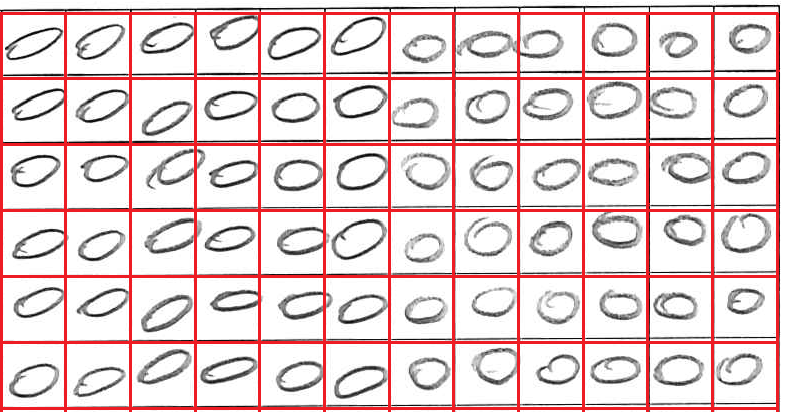
\includegraphics[width  =\textwidth]{figure/kiddi-01-grid-nosmooth-300dpi_cut.png}
\end{figure}

This could be caused from imprecise corner files, or some form of error when scanning the pages. \\


